\documentclass[border=2pt]{standalone}
\usepackage{pgfplots}
\pgfplotsset{compat=1.18}
\usepackage[T1]{fontenc}
\usepackage{times}
\begin{document}
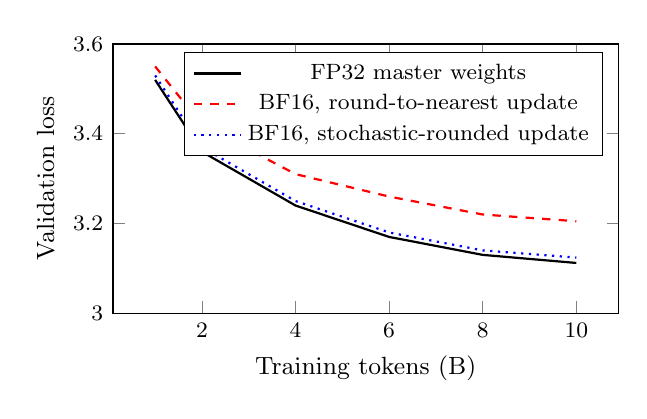
\begin{tikzpicture}
\begin{axis}[width=8cm,height=5cm,xlabel={Training tokens (B)},ylabel={Validation loss},
  legend style={font=\footnotesize,at={(0.97,0.97)},anchor=north east},
  tick label style={font=\footnotesize},label style={font=\small},ymin=3.0,ymax=3.6]
\addplot[thick,black] coordinates {(1,3.52) (2,3.36) (4,3.24) (6,3.17) (8,3.13) (10,3.112)};
\addlegendentry{FP32 master weights}
\addplot[thick,red,dashed] coordinates {(1,3.55) (2,3.42) (4,3.31) (6,3.26) (8,3.22) (10,3.205)};
\addlegendentry{BF16, round-to-nearest update}
\addplot[thick,blue,dotted] coordinates {(1,3.53) (2,3.37) (4,3.25) (6,3.18) (8,3.14) (10,3.124)};
\addlegendentry{BF16, stochastic-rounded update}
\end{axis}
\end{tikzpicture}
\end{document}
